\documentclass{project}

%---------- Edit for current document 
\usepackage[pdfauthor={Lars H Lunde},pdftitle={Test Specification Formal Review},pdftex]{hyperref}
\usepackage[pdftex]{graphicx}
\usepackage{wrapfig}

\begin{document}
\title{Group Project 14 - User manual}

%---------- Edit for current document 
\subtitle{User Manual}
\author{Lars H Lunde}     
\shorttitle{User Manual}
\version{0.1}
\status{Draft}
\date{2014-01-30}
\configref{GP14-USERMANUAL-01}

\maketitle
\tableofcontents
\newpage

%------------------- Document text
%-------- This section and its 3 subsections are mandatory for ANY document

\section{INTRODUCTION}

\subsection{Purpose of this Document}
To give the user an overview of how to use the application for its intended use.

\subsection{Scope}
This document covers how the application should be used, what each individual screen and button does. It also covers the results of each action in different conditions.

\subsection{Objectives}
This document should leave the user with the nescessary skills to operate the prgram for its intended purpose under all circumstances.

\clearpage

\section{THE APP}
\subsection{The start screen}

\begin{wrapfigure}{i}{0.7\textwidth}
  \begin{center}
    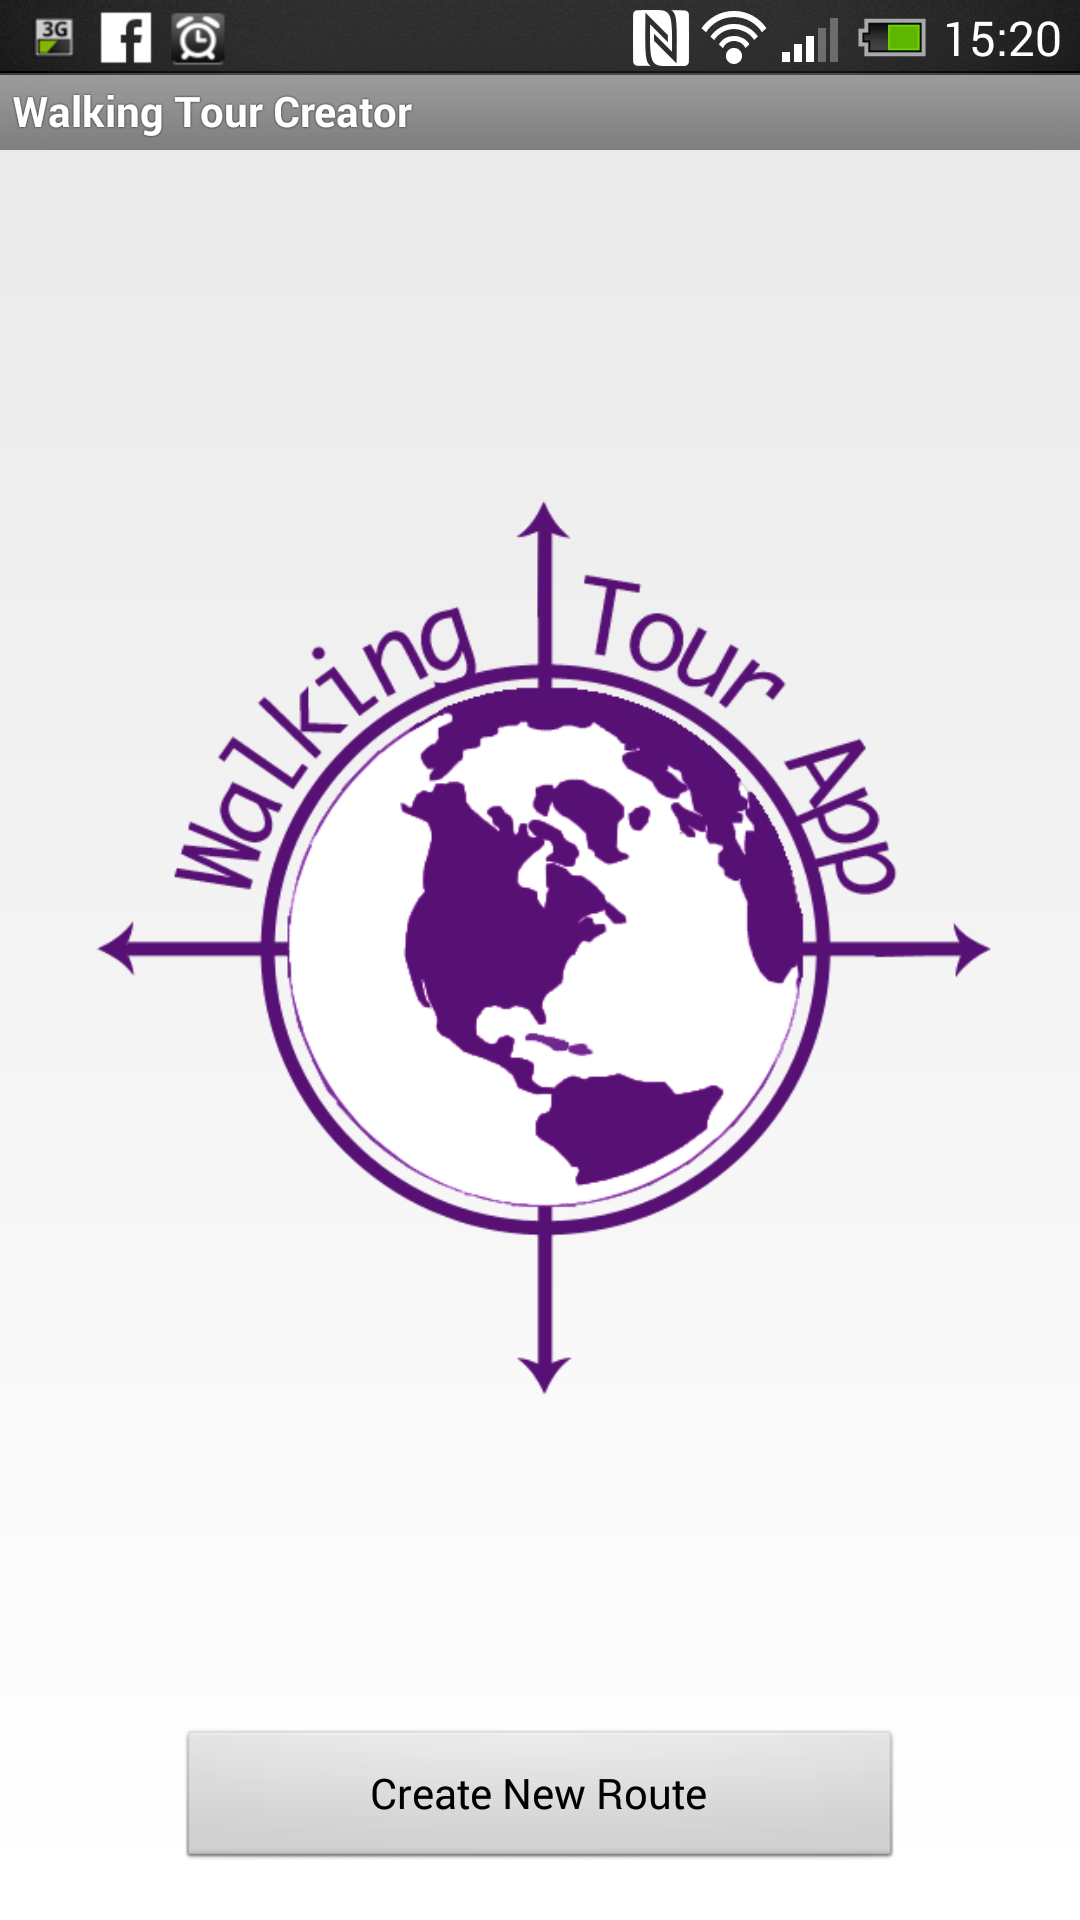
\includegraphics[width=0.7\textwidth]{front}
  \end{center}
\end{wrapfigure}

This is the welcoming screen of the application.
\newline
This only displays our apps logo and a button.
The button leads you to the screen letting you write the details of your walk.

\clearpage

\subsection{The walk details screen}

\begin{wrapfigure}{i}{0.5\textwidth}
  \begin{center}
    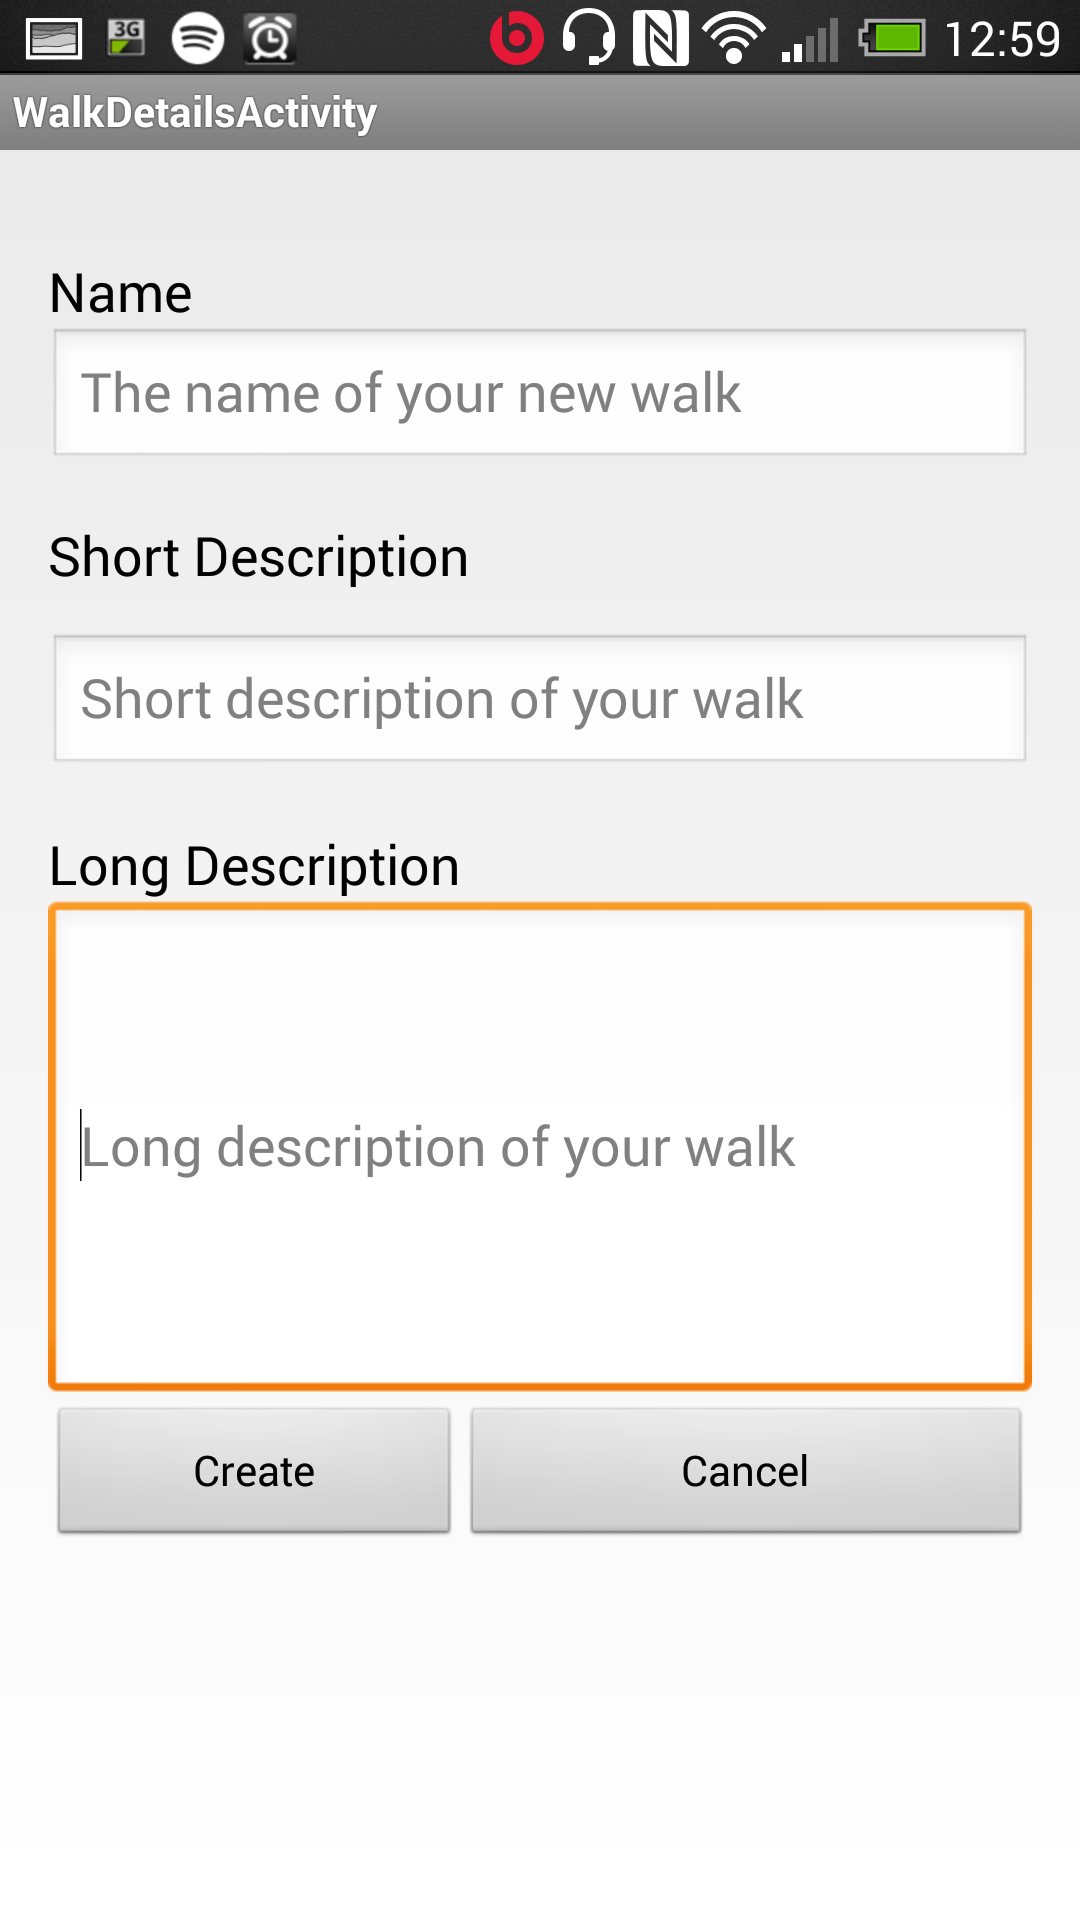
\includegraphics[width=0.7\textwidth]{details}
  \end{center}
\end{wrapfigure}

On this screen you choose what the name or "keyword" of the walk will be, give a short description of the walk  and a long description of the walk. On this screen there are some vital details to keep in mind:


\begin{enumerate}
  \item All fields need to have text in them
  \item The name may not contain any spaces
  \item The name may not be longer then 255 characters
  \item The short description may not be longer then 100 characters
  \item The long description may not be longer then 1000 characters
\end{enumerate}

However if you forget any of these details a helpful error will appear.
You are also faced with 2 buttons, one which validates your input and takes you to the Route editor, and one that cancels the walk and takes you back to the welcome screen.

\clearpage

\subsection{The walk details screen}

\begin{wrapfigure}{i}{0.6\textwidth}
  \begin{center}
    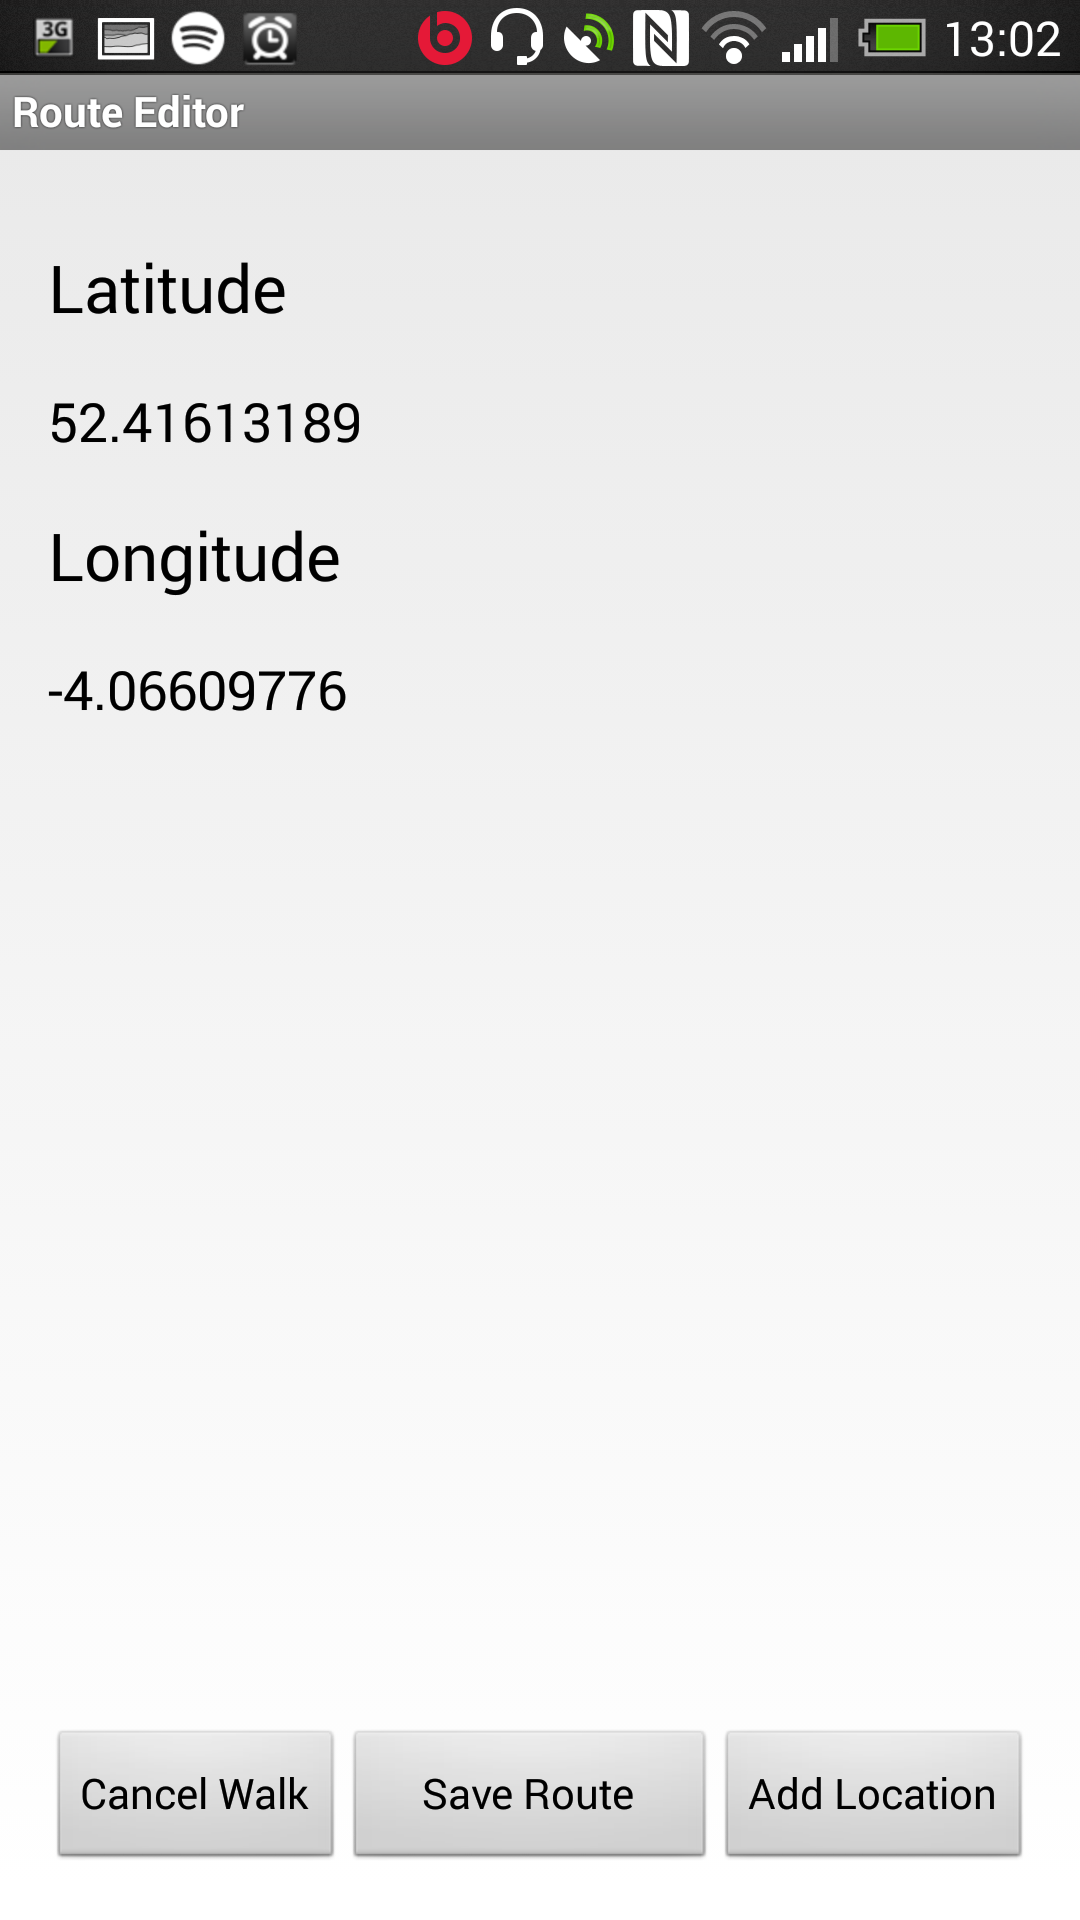
\includegraphics[width=0.6\textwidth]{route}
  \end{center}
\end{wrapfigure}

The route editor is the screen that will be active for most of the walk. Pressing back will have no effect, however you can press the home button and the app will run fine in the background. This screen will show you coordinates live on the screen as long as your GPS has a signal. If you do not have a signal, it will display 0.00000 on both values. 

You are also presented with 3 options, one to cancel the walk, one to Add a Location and one to save route.

Cancel walk is quite self explanatory, it will erase the current walk and take you back to the welcome page, however it will give you a warning before doing so.





%------------------- References
%--------- This contains  all the QA documents, edit out the ones you don't use in the document

\clearpage
\addcontentsline{toc}{section}{REFERENCES}
\begin{thebibliography}{5}

\bibitem{ReqSpec} \emph{Software Engineering Group Projects}
Walking Tour Creator Requirements Specification
C. J. Price, B.P.Tiddeman. 1.2 Release.

\bibitem{se.qa.01} \emph{Software Engineering Group Projects}
Quality Assurance Plan
C. J. Price, B.P.Tiddeman. 1.8 Release.

\bibitem{se.qa.02} \emph{Software Engineering Group Projects}
Project Management Standards
C. J. Price. 1.8 Release.

\bibitem{se.qa.03} \emph{Software Engineering Group Projects}
General Documentation Standards.
C. J. Price, N. W. Hardy. 1.5 Release.

\bibitem{se.qa.05A} \emph{Software Engineering Group Projects}
Design Specification Standards.
C. J. Price, N. W. Hardy, B.P.Tiddeman. 1.7 Release.

\bibitem{se.qa.05B} \emph{Software Engineering Group Projects}
Project Plan Specification Standards.
B.P.Tiddeman. 1.2 Release.

\bibitem{se.qa.06} \emph{Software Engineering Group Projects}
Test Procedure Standards.
C. J. Price, N.W.Hardy, B.P.Tiddeman. 1.7 Release.

\bibitem{se.qa.06} \emph{Software Engineering Group Projects}
Review Standards.
C. J. Price, N.W.Hardy, B.P.Tiddeman. 1.6 Release.

\bibitem{se.qa.08} \emph{Software Engineering Group Projects}
Operating Procedures and Configuration Management Standards
C. J. Price. 1.81 Release.

\bibitem{se.qa.09} \emph{Software Engineering Group Projects}
Java Coding Standards
C. J. Price, A. McManus. 1.7 Release.

\bibitem{se.qa.11} \emph{Software Engineering Group Projects}
Producing a Final Report
C. J. Price, N.W. Hardy, B.P.Tiddeman. 1.7 Release.

\end{thebibliography}

%---------------------- Version History 
\addcontentsline{toc}{section}{DOCUMENT HISTORY}
\section*{DOCUMENT HISTORY}
\begin{flushleft}
\begin{tabular}{ | p{1.5cm} | p{1cm} | p{2cm} | p{6cm}| p{1.5cm}| }
\hline
Version & CCF No. & Date & Changes made to Document & Changed by \\
\hline

%----------- Add edits and change author
0.1 & N/A & 2013-11-11 & Initial creation & lah25 \\
\hline

\end{tabular}
\end{flushleft}
\label{thelastpage}
\end{document}
